%%%%%%%%%%%%%%%%%%%%%%%%%%%%%%%%%%%%%%%%%%%%%%%%%%%%%%%%%%%%%%%%%%%%%%%%
%%%  THIS TEX FILE IS TO GENERATE PDF FILE FOR 
%%% 
%%%  COPYRIGHT (C) JIMMY LIN, 2013, UT AUSTIN
%%%%%%%%%%%%%%%%%%%%%%%%%%%%%%%%%%%%%%%%%%%%%%%%%%%%%%%%%%%%%%%%%%%%%%%%
\documentclass[11pt,a4paper]{article}
%%%%%%%%%%%%%%%%%%%%%%%%%%%%%%%%%%%%%%%%%%%%%%%%%%%%%%%%%%%%%%%%%%%%%%%%
%%%  PACKAGES USED IN THIS TEX SOURCE FILE
%%%%%%%%%%%%%%%%%%%%%%%%%%%%%%%%%%%%%%%%%%%%%%%%%%%%%%%%%%%%%%%%%%%%%%%%
\usepackage{geometry,amsthm,amsmath,graphicx,amssymb,fancyheadings}
\usepackage[]{mcode}
\usepackage[colorlinks,
            linkcolor=blue,
            anchorcolor=red,
            citecolor=green
            ]{hyperref}
% for my mac
\IfFileExists{/Users/JimmyLin/.latex/UTA_CS/JS.sty}{ 
    \usepackage{/Users/JimmyLin/.latex/UTA_CS/JS}
    \usepackage{/Users/JimmyLin/.latex/UTA_CS/JSASGN}
}{} 
% for UT's linux machine
\IfFileExists{/u/jimmylin/workspace/Configs/latex/UTA_CS/JS.sty}{
    \usepackage{/u/jimmylin/.latex/UTA_CS/JS} 
    \usepackage{/u/jimmylin/.latex/UTA_CS/JSASGN}
}{} 
%%%%%%%%%%%%%%%%%%%%%%%%%%%%%%%%%%%%%%%%%%%%%%%%%%%%%%%%%%%%%%%%%%%%%%%%
%%% MACROS CONTAINING THE FILE INFORMATION
%%%%%%%%%%%%%%%%%%%%%%%%%%%%%%%%%%%%%%%%%%%%%%%%%%%%%%%%%%%%%%%%%%%%%%%%
\renewcommand{\COURSE}{EE381V Large Scale Optimization}
\renewcommand{\LECTURER}{Sujay Sanghavi}
\renewcommand{\SECTION}{17350}
\renewcommand{\TASK}{Problem Set 2}
\renewcommand{\RELEASEDATE}{September 12, 2014}
\renewcommand{\DUEDATE}{September 18, 2014}
\renewcommand{\TIMECONSUME}{10 hours}
%%%%%%%%%%%%%%%%%%%%%%%%%%%%%%%%%%%%%%%%%%%%%%%%%%%%%%%%%%%%%%%%%%%%%%%%
%%% DOCUMENTATION STARTS FROM HERE 
%%%%%%%%%%%%%%%%%%%%%%%%%%%%%%%%%%%%%%%%%%%%%%%%%%%%%%%%%%%%%%%%%%%%%%%%
\begin{document}
%%%%%%%%%%%%%%%%%%%%%%%%%%%%%%%%%%%%%%%%%%%%%%%%%%%%%%%%%%%%%%%%%%%%%%%%
%% TITLE PAGE
%%%%%%%%%%%%%%%%%%%%%%%%%%%%%%%%%%%%%%%%%%%%%%%%%%%%%%%%%%%%%%%%%%%%%%%%
\begin{titlepage}
    \maketitle
\end{titlepage}
%%%%%%%%%%%%%%%%%%%%%%%%%%%%%%%%%%%%%%%%%%%%%%%%%%%%%%%%%%%%%%%%%%%%%%%%
%% CONTENT PAGE: TABLEOFCONTENTS, LISTOFTABLES, LIST OF FIGURES
%%%%%%%%%%%%%%%%%%%%%%%%%%%%%%%%%%%%%%%%%%%%%%%%%%%%%%%%%%%%%%%%%%%%%%%%
\renewcommand{\contentsname}{Table of Contents}
\begin{center} 
    \tableofcontents 
    %\listoftables 
    \listoffigures
\end{center}
\newpage
%%%%%%%%%%%%%%%%%%%%%%%%%%%%%%%%%%%%%%%%%%%%%%%%%%%%%%%%%%%%%%%%%%%%%%%%
%%% GENERAL DOCUMENTATION BEGINS 
%%%%%%%%%%%%%%%%%%%%%%%%%%%%%%%%%%%%%%%%%%%%%%%%%%%%%%%%%%%%%%%%%%%%%%%%
\newtheorem{remark}{Remark}
\part{Matlab and Computational Assignment}
\section{Five flavors for Eq. (9.20) in B \& V}
\subsection{Standard Gradient Descent with Backtracking}
{\bf Command} to be executed in matlab:
\begin{verbatim}
  >> x_init = [1 1]'; alpha = 0.3; bta = 0.8;
  >> [x, iter, all_costs] = gd_btls(x_init, @func, @func_grad, alpha, bta);
\end{verbatim}
{\bf Dump}
\begin{verbatim}
  Iter: 1, Cost: 5.292007e+00, Conv_Rate: 0.106142, gamma: 0.800000
  Iter: 2, Cost: 3.936296e+00, Conv_Rate: 0.743819, gamma: 0.409600
  Iter: 3, Cost: 3.440868e+00, Conv_Rate: 0.874138, gamma: 0.327680
  Iter: 4, Cost: 3.047567e+00, Conv_Rate: 0.885697, gamma: 0.262144
  Iter: 5, Cost: 2.851476e+00, Conv_Rate: 0.935657, gamma: 0.262144
  Iter: 6, Cost: 2.698084e+00, Conv_Rate: 0.946206, gamma: 0.209715
  Iter: 7, Cost: 2.621951e+00, Conv_Rate: 0.971783, gamma: 0.134218
  Iter: 8, Cost: 2.589490e+00, Conv_Rate: 0.987619, gamma: 0.107374
  Iter: 9, Cost: 2.571558e+00, Conv_Rate: 0.993075, gamma: 0.068719
                                ...
                                ...
  Iter: 40, Cost: 2.559267e+00, Conv_Rate: 1.000000, gamma: 0.000000
  Iter: 41, Cost: 2.559267e+00, Conv_Rate: 1.000000, gamma: 0.000000
  Iter: 42, Cost: 2.559267e+00, Conv_Rate: 1.000000, gamma: 0.000000
  Iter: 43, Cost: 2.559267e+00, Conv_Rate: 1.000000, gamma: 0.000000
  Iter: 44, Cost: 2.559267e+00, Conv_Rate: 1.000000, gamma: 0.000000
  Convergence reached!
\end{verbatim}
{\bf Minima}
\begin{verbatim}
    x = [-0.3379, -0.0031], obj = 2.559267 
   \end{verbatim}
{\bf Plot}
\begin{figure}[h]
    \centering
    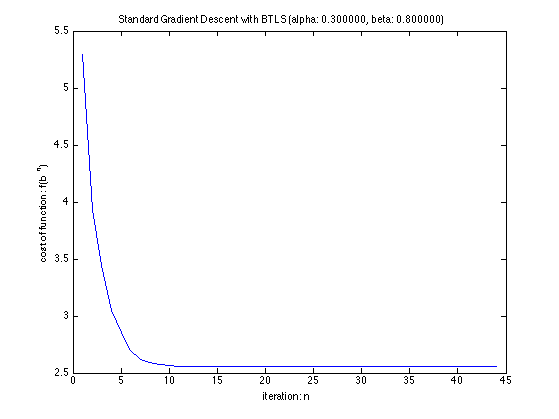
\includegraphics[width=4.6in,height=2.8in]{../ps2_matlab/1.png}
    \caption{Standard gradient descent with BTLS on
        Eq. 9.20 with $\alpha = 0.3$ and $\beta = 0.8$}
\end{figure}

\newpage
\subsection{Steepest Descent with $P_1$}
{\bf Command} to be executed in matlab:
\begin{verbatim}
  >> P1 = [8 0; 0 2];
  >> x_init = [1 1]'; alpha = 0.3; bta = 0.8;
  >> [x, iter, all_costs] = sd_btls(x_init, @func, @func_grad, P1, alpha, bta);
\end{verbatim}
{\bf Dump}
\begin{verbatim}
  Iter: 1, Cost: 4.109800e+00, Conv_Rate: 0.082430, gamma: 0.035184
  Iter: 2, Cost: 2.574134e+00, Conv_Rate: 0.626340, gamma: 0.409600
  Iter: 3, Cost: 2.561394e+00, Conv_Rate: 0.995051, gamma: 1.000000
  Iter: 4, Cost: 2.559319e+00, Conv_Rate: 0.999190, gamma: 0.800000
  Iter: 5, Cost: 2.559268e+00, Conv_Rate: 0.999980, gamma: 0.800000
  Iter: 6, Cost: 2.559267e+00, Conv_Rate: 1.000000, gamma: 0.800000
  Iter: 7, Cost: 2.559267e+00, Conv_Rate: 1.000000, gamma: 0.800000
  Iter: 8, Cost: 2.559267e+00, Conv_Rate: 1.000000, gamma: 0.800000
  Iter: 9, Cost: 2.559267e+00, Conv_Rate: 1.000000, gamma: 0.800000
  Iter: 10, Cost: 2.559267e+00, Conv_Rate: 1.000000, gamma: 0.800000
  Iter: 11, Cost: 2.559267e+00, Conv_Rate: 1.000000, gamma: 0.800000
  Iter: 12, Cost: 2.559267e+00, Conv_Rate: 1.000000, gamma: 1.000000
  Convergence reached!
\end{verbatim}
{\bf Minima}
\begin{verbatim}
    x = [-0.3466 -0.0000], obj = 2.559267 
   \end{verbatim}
{\bf Plot}
\begin{figure}[h]
    \centering
    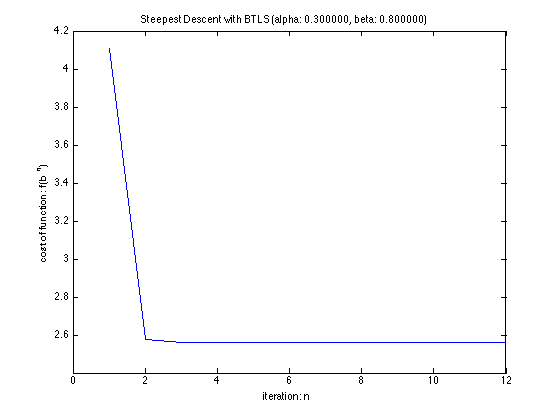
\includegraphics[width=5in,height=3in]{../ps2_matlab/2.png}
    \caption{Steepest Descent with BTLS on
        Eq. 9.20 with $P_1$, $\alpha = 0.3$ and $\beta = 0.8$}
\end{figure}

\newpage 
\subsection{Steepest Descent with $P_2$}
{\bf Command} to be executed in matlab:
\begin{verbatim}
  >> P2 = [2 0; 0 8];
  >> x_init = [1 1]'; alpha = 0.3; bta = 0.8;
  >> [x, iter, all_costs] = sd_btls(x_init, @func, @func_grad, P2, alpha, bta);
\end{verbatim}
{\bf Dump}
\begin{verbatim}
  Iter: 1, Cost: 5.397521e+00, Conv_Rate: 0.108258, gamma: 0.011529
  Iter: 2, Cost: 4.867283e+00, Conv_Rate: 0.901763, gamma: 0.068719
  Iter: 3, Cost: 4.673428e+00, Conv_Rate: 0.960172, gamma: 0.107374
  Iter: 4, Cost: 4.447617e+00, Conv_Rate: 0.951682, gamma: 0.085899
  Iter: 5, Cost: 4.276423e+00, Conv_Rate: 0.961509, gamma: 0.134218
  Iter: 6, Cost: 4.100684e+00, Conv_Rate: 0.958905, gamma: 0.107374
  Iter: 7, Cost: 3.955941e+00, Conv_Rate: 0.964703, gamma: 0.134218
  Iter: 8, Cost: 3.820349e+00, Conv_Rate: 0.965724, gamma: 0.134218
  Iter: 9, Cost: 3.687908e+00, Conv_Rate: 0.965333, gamma: 0.134218
  Iter: 10, Cost: 3.560463e+00, Conv_Rate: 0.965442, gamma: 0.134218
  Iter: 11, Cost: 3.444372e+00, Conv_Rate: 0.967394, gamma: 0.134218
  Iter: 12, Cost: 3.347890e+00, Conv_Rate: 0.971989, gamma: 0.167772
  Iter: 13, Cost: 3.259404e+00, Conv_Rate: 0.973570, gamma: 0.167772
                                ...
                                ...
  Iter: 164, Cost: 2.559267e+00, Conv_Rate: 1.000000, gamma: 0.262144
  Iter: 165, Cost: 2.559267e+00, Conv_Rate: 1.000000, gamma: 0.409600
  Iter: 166, Cost: 2.559267e+00, Conv_Rate: 1.000000, gamma: 0.327680
  Iter: 167, Cost: 2.559267e+00, Conv_Rate: 1.000000, gamma: 0.262144
  Iter: 168, Cost: 2.559267e+00, Conv_Rate: 1.000000, gamma: 0.167772
  Convergence reached!
\end{verbatim}
{\bf Minima}
\begin{verbatim}
    x = [-0.3466 -0.0000], obj = 2.559267
   \end{verbatim}
{\bf Plot}
\begin{figure}[h]
    \centering
    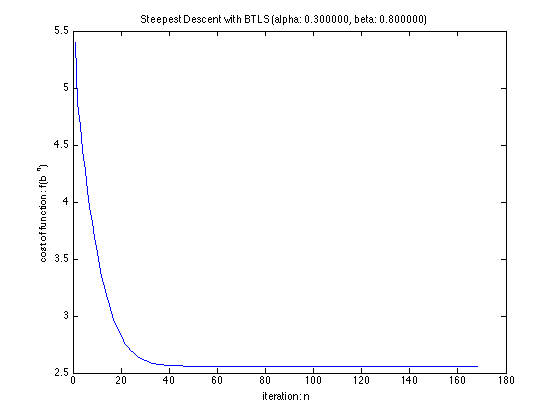
\includegraphics[width=5in,height=3in]{../ps2_matlab/3.png}
    \caption{Steepest Descent with BTLS on
        Eq. 9.20 with $P_2$, $\alpha = 0.3$ and $\beta = 0.8$}
\end{figure}

\newpage
\subsection{Cyclic Coordinate Descent}
{\bf Command} to be executed in matlab:
\begin{verbatim}
  >> x_init = [1 1]'; alpha = 0.3; bta = 0.8;
  >> [x, iter, all_costs] = ccd_btls(x_init, @func, @func_grad, alpha, bta);
\end{verbatim}
{\bf Dump}
\begin{verbatim}
  Iter: 1, Cost: 1.217687e+01, Conv_Rate: 0.244232, gamma: 0.043980
  Iter: 2, Cost: 3.551842e+00, Conv_Rate: 0.071239, gamma: 0.035184
  Iter: 3, Cost: 3.064142e+00, Conv_Rate: 0.862691, gamma: 0.209715
  Iter: 4, Cost: 2.732279e+00, Conv_Rate: 0.769257, gamma: 0.134218
  Iter: 5, Cost: 2.664867e+00, Conv_Rate: 0.975328, gamma: 0.209715
  Iter: 6, Cost: 2.600923e+00, Conv_Rate: 0.951925, gamma: 0.134218
  Iter: 7, Cost: 2.585633e+00, Conv_Rate: 0.994121, gamma: 0.262144
  Iter: 8, Cost: 2.563802e+00, Conv_Rate: 0.985727, gamma: 0.107374
  Iter: 9, Cost: 2.561867e+00, Conv_Rate: 0.999245, gamma: 0.209715
  Iter: 10, Cost: 2.560171e+00, Conv_Rate: 0.998584, gamma: 0.107374
  Iter: 11, Cost: 2.559836e+00, Conv_Rate: 0.999869, gamma: 0.167772
  Iter: 12, Cost: 2.559551e+00, Conv_Rate: 0.999758, gamma: 0.107374
  Iter: 13, Cost: 2.559478e+00, Conv_Rate: 0.999971, gamma: 0.167772
                                ...
                                ...
  Iter: 60, Cost: 2.559267e+00, Conv_Rate: 1.000000, gamma: 0.134218
  Iter: 61, Cost: 2.559267e+00, Conv_Rate: 1.000000, gamma: 0.262144
  Iter: 62, Cost: 2.559267e+00, Conv_Rate: 1.000000, gamma: 0.085899
  Iter: 63, Cost: 2.559267e+00, Conv_Rate: 1.000000, gamma: 0.327680
  Iter: 64, Cost: 2.559267e+00, Conv_Rate: 1.000000, gamma: 0.134218
  Convergence reached!
\end{verbatim}
{\bf Minima}
\begin{verbatim}
    x = [-0.3466 0.0000], obj = 2.559267 
   \end{verbatim}
{\bf Plot}
\begin{figure}[h]
    \centering
    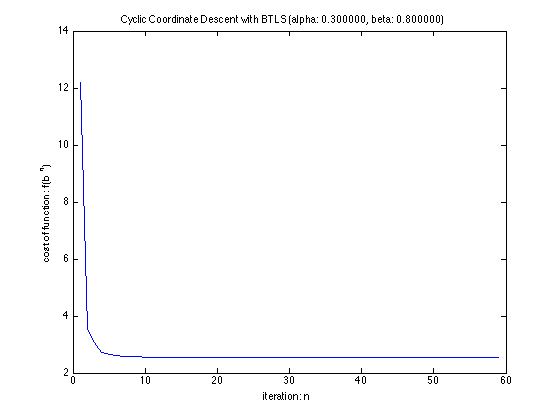
\includegraphics[width=5in,height=3in]{../ps2_matlab/4.png}
    \caption{Cyclical Coordinate Descent with BTLS on
        Eq. 9.20 with $\alpha = 0.3$ and $\beta = 0.8$}
\end{figure}
\newpage
\subsection{Greedy Coordinate Descent}
{\bf Command} to be executed in matlab:
\begin{verbatim}
  >> x_init = [1 1]'; alpha = 0.3; bta = 0.8;
  >> [x, iter, all_costs] = gcd_btls(x_init, @func, @func_grad, alpha, bta);
\end{verbatim}
{\bf Dump}
\begin{verbatim}
Iter: 1, Cost: 5.615225e+00, Conv_Rate: 0.112625, gamma: 0.005903
Iter: 2, Cost: 4.227075e+00, Conv_Rate: 0.752788, gamma: 0.028147
Iter: 3, Cost: 3.306101e+00, Conv_Rate: 0.782125, gamma: 0.035184
Iter: 4, Cost: 2.823271e+00, Conv_Rate: 0.853958, gamma: 0.054976
Iter: 5, Cost: 2.666299e+00, Conv_Rate: 0.944401, gamma: 0.068719
Iter: 6, Cost: 2.577867e+00, Conv_Rate: 0.966834, gamma: 0.107374
Iter: 7, Cost: 2.566546e+00, Conv_Rate: 0.995608, gamma: 0.107374
Iter: 8, Cost: 2.561822e+00, Conv_Rate: 0.998160, gamma: 0.107374
Iter: 9, Cost: 2.560570e+00, Conv_Rate: 0.999511, gamma: 0.107374
Iter: 10, Cost: 2.559369e+00, Conv_Rate: 0.999531, gamma: 0.107374
Iter: 11, Cost: 2.559298e+00, Conv_Rate: 0.999972, gamma: 0.107374
Iter: 12, Cost: 2.559277e+00, Conv_Rate: 0.999992, gamma: 0.107374
                                ...
                                ...
Iter: 32, Cost: 2.559267e+00, Conv_Rate: 1.000000, gamma: 0.107374
Iter: 33, Cost: 2.559267e+00, Conv_Rate: 1.000000, gamma: 0.107374
Iter: 34, Cost: 2.559267e+00, Conv_Rate: 1.000000, gamma: 0.107374
Iter: 35, Cost: 2.559267e+00, Conv_Rate: 1.000000, gamma: 0.107374
Convergence reached!
\end{verbatim}
{\bf Minima}
\begin{verbatim}
    x = [-0.3466 -0.0000], obj = 2.559267 
   \end{verbatim}
{\bf Plot}
\begin{figure}[h]
    \centering
    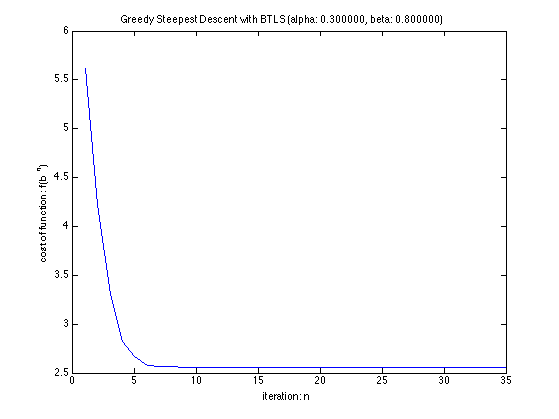
\includegraphics[width=5in,height=3in]{../ps2_matlab/5.png}
    \caption{Greedy Coordinate Descent with BTLS on
        Eq. 9.20 with $\alpha = 0.3$ and $\beta = 0.8$}
\end{figure}

\newpage
\subsection{Conclusions}
\begin{itemize}
    \item $(1, 1)$ is an decent initial point for all five
        flavors of optimization methods.
    \item Steepest descent method could both enhance and impair the convergence
        speed, comparing to standard gradient descent (uniform heuristic or
        unheuristic). The specific effect depends on what heuristic matrix is provided. 
    \item Greedy coordinate descent does converge to optima in less number of
        iterations than the cyclic cooridnate descent but in larger
        computational cost in each iteration.
\end{itemize}

%%%%%%%%%%%%%%%%%%%%%%%%%%%%%%%%%%%%%%%%%%%%%%%%%%%%%%%%%%%%
%%% Written Problems
%%%%%%%%%%%%%%%%%%%%%%%%%%%%%%%%%%%%%%%%%%%%%%%%%%%%%%%%%%%%
\newpage
\part{Written Problems}
\setcounter{section}{0}
\renewcommand{\thesubsection}{(\alph{subsection})}
\section{Coordinate Descent}
\subsection{Give an example}
The example to illustrate failure of coordinate descent in converging to
global minimum of function $f$ at point $x$ is
\begin{align}
    f(x,y) = || (x,y) ||_{\infty} = max (x, y)
\end{align}
at point $(x,y) = (-2, -2)$. \\
And the contour is drawn as follows:
\begin{figure}[h]
    \centering
    \includegraphics[width=4in]{./coordinate_descent.png}
    \caption{Contour of function $f(x,y) = || (x,y) ||_{\infty}$}
\end{figure}

\noindent
Note that since $f(x,y) = || (x,y) ||_{\infty}$ is not differentiable, any
coordinate descent that employs gradient of $f(x,y)$ is not available. But we
can still apply non-gradient-based coordinate descent algorithm on this
problem. 

\begin{remark}
    There is a bug for this question. Function can be chosen as $f(x) = x$, which
    is convex but not strongly convex and the point $x$ can be arbitrary
    point. Since $f(x) = x$ has its global minimum $-\infty$, then the
    coordinate descent starting from arbitrary point $x \in \mathbb{R}$ can  
    never get to the global minimum of $f$ forever. 
\end{remark}

\subsection{$f(x,y) = x^2 + y^2 + 3xy$}
The coordinate descent with exact line search {\bf will not} always
converge to a stationary point. The stationary point is $(x,y) = (0, 0)$.
Consider the coordinate descent at $(10, -10)$: 
\begin{align}
    \frac{\partial f(x,y)}{\partial x} &= 2x + 3y = -10 
    && f(x,y) \text{ will descend if } x \text{ increase} \\
    \frac{\partial f(x,y)}{\partial y} &= 2y + 3x = 10
    && f(x,y) \text{ will descend if } y \text{ decrease}
\end{align}
Obviously, the coordinate descent at $(10, -10)$ will go away from $(0,0)$.
Therefore, $f(x,y)$ has no guarantee to converge to stationary point by
coordinate descent with exact line search.

%%%%%%%%%%%%%%%%%%%%%%%%%%%%%%%%%%%%%%%%%%%%%%%%%%%%%%%%%%%%
\newpage
\section{Condition Number}
For arbitrary step size $t$, the strongly convex function $f(x) = \frac{1}{t}
x^2$ starting from $x_0 = 1$ does not converge to optimal solution. 

\begin{proof}
    We begin with showing $f(x) = \frac{1}{t} x^2$ is strongly convex.
    Obviously, $0 \leq f(x) \leq \frac{2}{t}$. 
    Hence, function $f(x) = \frac{1}{t} x^2$ is strongly convex with $m = 0$
    and $M = \frac{1}{t}$. (The hessian of $f(x)$ is bounded.)

    Then we show that $f(x) = \frac{1}{t} x^2$ starting from $x_0 = 1$ does
    not converge to optimal solution. The gradient of $f(x)$ at $x_0$ is given
    by
    \begin{align}
        \nabla f(x_0)
        = \nabla f(x)|_{x=1} 
        = \frac{2}{t} x |_{x=1} 
        = \frac{2}{t}
    \end{align}

    By gradient algorithm, the update direction at $x_0$ is given by
    \begin{align}
        \delta x_0 = - \nabla f(x_0) = \frac{2}{t}
    \end{align}

    Apply the update step
    \begin{align}
        x^{+} = x_0 - \Delta x_0 = 1 - t \cdot \frac{2}{t} = 1 - 2 = -1
    \end{align}

    It is obvious that 
    \begin{align}
        f(x^{+}) = f(-1) = \frac{1}{t}  = f(1) = f(x_0)
    \end{align}

    Continue the gradient algorithm repeatedly. And then we find that the function at
    $k$-step always equals its initial value $f(x_0)$ and never reach its optimum.
    \begin{align}
        f(x_{k}) = f (x_0) \not = f(0) = 0
    \end{align}

    Hence, it is proved that 
       {\it for any fixed step size $t$ , there exists a smooth
            strongly convex function with bounded Hessian, such that a fixed
            stepsize gradient algorithm starting from some point  $x_0$, does
            not converge to the optimal solution.}
\end{proof}

%%%%%%%%%%%%%%%%%%%%%%%%%%%%%%%%%%%%%%%%%%%%%%%%%%%%%%%%%%%%
\newpage
\section{Decreasing Stepsize}

\begin{proof}
    Let constant $m$ and $M$ be the lower and uppper bound on hessian of
    $f(x)$. That is 
    \begin{align}
        mI \leq \nabla^2 f(x) \leq MI
    \end{align}
    The given conditions are 
    \begin{align}
        \lim_{k\rightarrow \infty} t_k  = 0 \\
        \Sigma_{k=0}^{\infty} t_k = \infty
    \end{align}
    which tells us that $t_k$ will start from very large value and finally
    decrease to 0 (sufficiently small step size). Then we have 
    \begin{align}
        \exists k,\ 0 < t_k < \frac{1}{M} \label{above}
    \end{align}
    By second-order approximation and lower bound of Hessian on step $k$, we have 
    \begin{align}
        f(x_{k+1}) &\leq f(x) - t_k || f(x_k) ||_2^2 + \frac{Mt_k^2}{2} ||
        f(x_k) ||_2^2 \\
        f(x_{k+1}) &\leq f(x) (\frac{Mt_k}{2} - 1) t_k || f(x_k) ||_2^2 
    \end{align}
    In terms of \eqref{above}, then we have 
    \begin{align}
        f(x_{k+1}) \leq f(x_k) - \frac{1}{2} t_k || \nabla f(x_k) ||_2^2
    \end{align}
    Subtracted both sides with $p^*$
    \begin{align}
        f(x_{k+1}) - p^* \leq f(x_k) - p^* - \frac{1}{2} t_k || \nabla f(x_k) ||_2^2
    \end{align}
    Combined with previously derived inequality 
    \begin{align}
        || \nabla f(x_k) ||_2^2  \geq 2m \big( f(x) - p^* \big)
    \end{align}
    Then we have 
    \begin{align}
        f(x_{k+1}) - p^* \leq (1- m t_k ) (f(x_k) - p^*)  
    \end{align}
    Since $ m > 0 $ and $t_k > 0$, then 
    \begin{align}
        f(x_{k+1}) - p^* \leq c (f(x_k) - p^*)  
    \end{align}
    where $c = (1- m t_k ) < 1$. And let us apply this formula recursively
    and get
    \begin{align}
        f(x_{k+1}) - p^* \leq c^k (f(x_0) - p^*)  
    \end{align}
    which guarantee the convergence of $f(x)$ since $c < 1$.
    Hence, it can be concluded that with the
    infinity decreasing step size sequence, the gradient descent must converge to
    the global optimal solution. 
\end{proof}

%%%%%%%%%%%%%%%%%%%%%%%%%%%%%%%%%%%%%%%%%%%%%%%%%%%%%%%%%%%%
\newpage
\section{Convex Functions}
\subsection{$f(x) = \sup_i f_i (x)$}
Let $a$ and $b$ be two arbitrary distinct points such that $a \in dom f$ and $b \in dom f$. And
let $\lambda \in [0, 1]$.
\begin{align}
    f(\lambda a + (1-\lambda) b) 
    &= \sup_i f_i (\lambda a + (1-\lambda) b) \\
    &\leq \sup_i \lambda f_i (a) + (1-\lambda) f_i (b) \\
    &\leq \sup_i \lambda f_i (a) + \sup_i (1-\lambda) f_i (b) \\
    &= \lambda \sup_i  f_i (a) + (1-\lambda) \sup_i f_i (b) \\
    &= \lambda f(a) + (1-\lambda) f(b)
\end{align}
Since $ f(\lambda a + (1-\lambda) b) \leq \lambda f(a) + (1-\lambda) f(b)$
hold for arbitrary distinct points $a$ and $b$, we
can conclude that 
\begin{align}
    f_i(x) \text{ is convex } \forall i \Rightarrow f(x) = \sup_i f_i(x) \text{ is convex. }
\end{align}

\subsection{$\lambda_{max} (M)$}
Let $M_1$ and $M_2$ be arbitrarily distinct matrix of the same dimensionality.
Let $v_0$, $v_1$, $v_2$ be eigen vector of $\alpha M_1 + (1-\alpha) M_2$,
$M_1$ and $M_2$ respectively. 
and let $\lambda_0$, $\lambda_1$, $\lambda_2$ be the largest eigen value of $\alpha M_1 +
(1-\alpha) M_2$, $M_1$ and $M_2$ respectively. $\alpha \in [0, 1]$. 
By eigenvalue decomposition, we have
\begin{align}
    v_1^T M_1 v_1 = \lambda_1     \\
    v_2^T M_2 v_2 = \lambda_2     \\
    v_0^T \big(\alpha M_1 + (1-\alpha) M_2 \big) v_0 = \lambda_0   
\end{align}
It is obvious that 
\begin{align}
    v_1^T M_1 v_1 = v_0^T M_1 v_0     \\
    v_2^T M_2 v_2 = v_0^T M_2 v_0   
\end{align}
Otherwise, $\lambda_0$, $\lambda_2$, $\lambda_2$ cannot be the largest eigen
value. \\
Then we have
\begin{align}
    \alpha v_1^T M_1 v_1 \geq \alpha v_0^T M_1 v_0     \\
    (1-\alpha) v_2^T M_2 v_2 \geq (1-\alpha) v_0^T M_2 v_0   
\end{align}
Add above two inequalities up, we have
\begin{align}
    \alpha v_1^T M_1 v_1 + (1-\alpha) v_2^T M_2 v_2 
    \geq \alpha v_0^T M_1 v_0  + (1-\alpha) v_0^T M_2 v_0
\end{align}
That is 
\begin{align}
    \alpha \lambda_1 + (1-\alpha) \lambda_2 
    \geq v_0^T(\alpha M_1 + (1-\alpha) M_2) v_0 = \lambda_0
\end{align}
Hence, we can conclude that function $\lambda_{max}$ is convex. \\
\begin{remark}
    The eigenvalue of largest magnitude is not convex.
\end{remark}
\newpage
\subsection{Weighted shortest path from $a$ to $b$}
For a fixed graph topology with distinct weights $w_1$ and $w_2$, we have
\begin{align}
    \lambda f(w_1) + (1-\lambda) f(w_2)
    = f(\lambda w_1) + f((1-\lambda) w_2)
\end{align}
where $\lambda$ is abitrary real value between 0 and 1. The above step is valid
because if we multiply every weight of edge with a constant ($\lambda$ in this
case), then the path between two nodes with minimal weights stay invariant and
hence minimal weights of that path becomes a constant ($\lambda$) multiple of
its original value.
\begin{align}
    f(\lambda w_1) + f((1-\lambda) w_2)
    \leq f(\lambda w_1 + (1-\lambda) w_2)  
\end{align}
    To simplify the explanation, we denote the cost of minimal-weight path
    returned by $f(\lambda w_1 + (1-\lambda) w_2)$ under weight $w$ as
    $PC(w)$). That is to say,  
\begin{align}
    f(\lambda w_1 + (1-\lambda) w_2) = PC(\lambda w_1) + PC((1-\lambda) w_2)
\end{align}
    The justification is as follows:
\begin{itemize}
    \item If $f(\lambda w_1)$ and $f((1-\lambda) w_2)$ return different
        paths between two nodes,  then by definition we have
        $f(\lambda w_1) \leq PC(\lambda w_1)$ and 
        $f((1-\lambda) w_2) \leq PC((1-\lambda) w_2)$. Sum up these two
        inequalities derives $f(\lambda w_1) + f((1-\lambda) w_2) < f(\lambda w_1 + (1-\lambda) w_2)$
    \item If $f(\lambda w_1)$ and $f((1-\lambda) w_2)$ return the same path
        between two nodes, it is obvious that the equality holds.
\end{itemize}
Hence, we have 
\begin{align}
    \lambda f(w_1) + (1-\lambda) f(w_2)
    \leq f(\lambda w_1 + (1-\lambda) w_2)  
\end{align}
which indicates that $f$ is concave function of $w$.

%%%%%%%%%%%%%%%%%%%%%%%%%%%%%%%%%%%%%%%%%%%%%%%%%%%%%%%%%%%%
\newpage
\section{Convex Functions: Jensen's Inequality}
\subsection{$epi(f)$ is also convex if $f(x)$ is convex}
Let $(a_1, b_1)$ and $(a_2, b_2)$ are two distinct pair that belongs to
$epi(f)$. That is 
\begin{align}
    a_1 \not = a_2 , b_1 \not = b_2 \\
    (a_1, b_1) \in epi(x) \label{pair1member} \\
    (a_2, b_2) \in epi(x) \label{pair2member}
\end{align}
We want to prove for arbitrary $\lambda \in [0, 1]$, 
\begin{align}
    \lambda(a_1, b_1) + (1-\lambda)(a_2, b_2) \in epi(x)
\end{align}
holds. \\
In terms of \eqref{pair1member} and \eqref{pair2member}, we have
\begin{align}
    b_1 \geq f(a_1) \\
    b_2 \geq f(a_2) 
\end{align}
Multiply both sides with $\lambda$ and $(1-\lambda)$ respectively
\begin{align}
    \lambda b_1 &\geq \lambda f(a_1) \\
    (1-\lambda) b_2 &\geq (1-\lambda) f(a_2) 
\end{align}
Then add up two terms above, we have
\begin{align}
    \lambda b_1 + (1-\lambda) b_2 \geq \lambda f(a_1) + (1-\lambda) f(a_2) 
\end{align}
Since $f(x)$ is convex, then we have
\begin{align}
    \lambda f(a_1) + (1-\lambda) f(a_2) \geq f (a_1 + (1-\lambda) a_2)
\end{align}
Then
\begin{align}
    \lambda b_1 + (1-\lambda) b_2 \geq \lambda f (a_1 + (1-\lambda) a_2)
\end{align}
That is to say,
\begin{align}
    (\lambda a_1 + (1-\lambda) a_2, \lambda b_1 + (1-\lambda) b_2) \in epi (f)
\end{align}
which can be written as 
\begin{align}
    \lambda(a_1, b_1) + (1-\lambda)(a_2, b_2) \in epi(f)
\end{align}
Hence, we can conclude that $epi(f)$ is a convex set.

\newpage
\subsection{Finite version of Jensen's inequality}
\newcommand{\E}{\mathbb{E}}
We prove this by induction on $m$.   \\
Base Case: $m = 1$. It is obvious that $\E(f(x_1)) = f(E(x_1)) = f(x_1)$. \\
Inductive Cases: assume that for $\sum_{i=1}^m p_i = 1$
\begin{align}
    \E[f(X_m)] &= \sum_{i=1}^m p_i f(x_i) \leq f(\sum_{i=1}^m p_i x_i) = f(\E(X_{m}))
\end{align}
holds and show that for $\sum_{i=1}^{m+1} p_i = 1$, 
\begin{align}
    \E[f(X_{m+1})] &= \sum_{i=1}^{m+1} p_i f(x_i) 
    \leq f(\sum_{i=1}^{m+1} p_i x_i) = f(\E(X_{m+1}))
\end{align}
is true.
\begin{proof}
    \begin{align}
        \E[f(X_{m+1})] &= \sum_{i=1}^{m} p_i f(x_i) + p_{m+1} f(x_i)  \\
        &= \big(\sum_{i=1}^{m} p_i \big) \sum_{i=1}^{m}
        \frac{p_i}{\sum_{i=1}^{m} p_i} f(x_i) + p_{m+1} f(x_{m+1})  \\
        &\leq \big(\sum_{i=1}^{m} p_i \big) f(\sum_{i=1}^{m}
        \frac{p_i}{\sum_{i=1}^{m} p_i} x_i) + p_{m+1} f(x_{m+1})  \\
        &\leq f \big( (\sum_{i=1}^{m} p_i) \sum_{i=1}^{m}
        \frac{p_i}{\sum_{i=1}^{m} p_i} x_i + p_{m+1} x_{m+1} \big) \\
        &= f \big( \sum_{i=1}^{m} p_i x_i + p_{m+1} x_{m+1} \big) \\
        &= f(\sum_{i=1}^{m+1} p_i x_i) \\
        &= f(\E(X_{m+1}))
    \end{align}
    Hence, it is proved that $\E[f(X_{m+1})] \leq f(\E(X_{m+1}))$. And the
    induction holds. 
\end{proof}
\noindent
From the base case and inductive cases, it can be concluded by induction that 
\begin{align}
    \E[f(X)] &  \leq f(\E(X))
\end{align}


%%%%%%%%%%%%%%%%%%%%%%%%%%%%%%%%%%%%%%%%%%%%%%%%%%%%%%%%%%%%
\newpage
\section{Projection}
We start by manipulating the solution. \\
By the definition of projection, we have 
\begin{align}
    x^{(k+1)} &= Proj_{\chi}(x^{(k)} - t_k \nabla f(x^{(k)})) \\
    &= argmin_{x\in \chi} || x - (x^{(k)} - t_k \nabla f(x^{(k)}) ) ||_2 \\
    &= argmin_{x\in \chi} || (x - x^{(k)}) + t_k \nabla f(x^{(k)}) ) ||_2^2 \\
    &= argmin_{x\in \chi} \big( || x - x^{(k)} ||_2^2 
       + 2 t_k (x - x^{(k)} ) \nabla f(x^{(k)}) 
       + t_k^2 || \nabla f(x^{(k)}) ||_2^2  \big) \\
    &= argmin_{x\in \chi} \big( || x - x^{(k)} ||_2^2 
       + 2 t_k x \nabla f(x^{(k)}) - 2 t_k x^{(k)}\nabla f(x^{(k)})   
       + t_k^2 || \nabla f(x^{(k)}) ||_2^2  \big)
\end{align}
Obviously, both $- 2 t_k x^{(k)}\nabla f(x^{(k)})$ and $t_k^2 || \nabla f(x^{(k)})
||_2^2$ are constant term at step $k$. Then, we can remove them in the optimization
objective.
\begin{align}
    x^{(k+1)} &= Proj_{\chi}(x^{(k)} - t_k \nabla f(x^{(k)})) \\
    &= argmin_{x\in \chi} \big( || x - x^{(k)} ||_2^2 
    + 2 t_k x \nabla f(x^{(k)})  \big) \\
    &= argmin_{x\in \chi} \big(  
     2 t_k \langle x, \nabla f(x^{(k)}) \rangle + || x - x^{(k)} ||_2^2 \big) \\
    &= argmin_{x\in \chi} \big(  \langle x, \nabla f(x^{(k)}) \rangle
    + \frac{1}{2t_k} || x - x^{(k)} ||_2^2 \big)
\end{align}
Note that the last step is valid because $t_k$ is constant at step $k$. \\
Hence, we proved that 
\begin{align}
x^{(k+1)} &= argmin_{x\in \chi} \big(  \langle x, \nabla f(x^{(k)}) \rangle
    + \frac{1}{2t_k} || x - x^{(k)} ||_2^2 \big) \\
    \Longleftrightarrow\ x^{(k+1)} &= Proj_{\chi}(x^{(k)} - t_k \nabla f(x^{(k)})) 
\end{align}
%%%%%%%%%%%%%%%%%%%%%%%%%%%%%%%%%%%%%%%%%%%%%%%%%%%%%%%%%%%%
\newpage
\section{Computing Projections}
\newcommand{\Rpn}{\mathbb{R}_+^n}
\newcommand{\Spn}{S_+^n}
\subsection{$\chi = \{x: L_i \leq x_i \leq U_i, i = 1, ..., n\}$}
\begin{align}
    argmin_{L_i \leq x_i \leq U_i} || x_i - z_i ||_2^2
\end{align}
Solving this objective, we get 
\begin{align}
x_i^{*} = max( min(z_i, U_i), L_i),\ \forall i
\end{align}
\subsection{$\chi = \Rpn$}
The solution is 
\begin{align}
x_i^{*} = max(z_i, L_i),\ \forall i
\end{align}
Note that we can simply view $\Rpn$ as rectangle with $L = 0$ and $U =
\infty$.
\subsection{Euclidean ball: $\{x: || x ||_2 \leq 1 \}$}
As to the Euclidean ball: $\{x: || x ||_2 \leq 1 \}$, we have projection task
as follows:
\begin{align}
    argmin_{|| x ||_2^2 \leq 1 } || x_i - z_i ||_2^2
\end{align}
Solving this by using lagrangian
\begin{align}
    L(x, \lambda) = || x - z ||_2 + \lambda (|| x ||_2^2 - 1)
\end{align}
And we get the stationary point by setting gradient to zero,
\begin{align}
    x = \frac{z}{1+\lambda}
\end{align}
Now we need to discuss the value of $x$ and $z$. If $|| z || \leq 1$, then
$\lambda = 0$. But if $|| z || > 1$, then $|| x ||_2 = \frac{z}{||z||_2}$.

\subsection{1-norm ball: $\{x: \Sigma_i | x_i | \leq 1 \}$}

\subsection{Positive semidefinite cone: $\Spn = \{ M \in S^n: x^T M x \geq 0,
        \forall x \in R^n \}$ }
\subsection{Probability Simplex: $\chi = \{\Sigma_i x_i = 1, x_i \geq 0, i =
        1, ..., n \}$}

%%%%%%%%%%%%%%%%%%%%%%%%%%%%%%%%%%%%%%%%%%%%%%%%%%%%%%%%%%%%
%%% Appendix
%%%%%%%%%%%%%%%%%%%%%%%%%%%%%%%%%%%%%%%%%%%%%%%%%%%%%%%%%%%%
\newpage
\appendix
\section{Codes Printout}

\subsection{Eq. 20 and its gradient}
\lstinputlisting{../ps2_matlab/func.m}
\lstinputlisting{../ps2_matlab/func_grad.m}

\newpage
\subsection{Standard Gradient Descent with BackTracking Line Search}
\lstinputlisting{../ps2_matlab/gd_btls.m}
\newpage

\subsection{Steepest Descent with BackTracking Line Search}
\lstinputlisting{../ps2_matlab/sd_btls.m}
\newpage

\subsection{Cyclic Coordinate Descent}
\lstinputlisting{../ps2_matlab/ccd_btls.m}
\newpage

\subsection{Greedy Coordinate Descent}
\lstinputlisting{../ps2_matlab/gcd_btls.m}
\newpage
%%%%%%%%%%%%%%%%%%%%%%%%%%%%%%%%%%%%%%%%%%%%%%%%%%%%%%%%%%%%%%%%%%%%%%%%
%%% General Documentation ends
%%%%%%%%%%%%%%%%%%%%%%%%%%%%%%%%%%%%%%%%%%%%%%%%%%%%%%%%%%%%%%%%%%%%%%%%
\end{document}
\subsubsection{Steepest Descent with $P_2$}
